\documentclass[tikz,border=2pt]{standalone}
\usepackage[T1]{fontenc}
\usepackage{lmodern}
\usetikzlibrary{arrows.meta,positioning,calc,fit,backgrounds}
% Spark processing scheme: the user application, the driver program with its
% SparkSession, logical plan, Catalyst optimizer, DAG and task schedulers and
% driver services, the cluster manager, the external storage, and the worker
% nodes whose executors hold a cache, tasks and a block manager, with a legend
% of the seven kinds of components. The style follows the figure of
% #fig_sparkApplicactions (figs/chap8/sparkApplicactions.tex); the seven kinds
% of the legend take light tints of seven hues. The figure is 14.2 cm wide in
% three tiers, the application above the driver program, the external storage
% and the cluster manager right of it, and the worker nodes below, so that,
% printed at the text width, its text keeps about 80% of the height of the
% caption, as the figure of the Spark SQL components (sparkArq.tex) does.
\colorlet{cuser}{blue!12}
\colorlet{cdriver}{violet!14}
\colorlet{cplan}{orange!16}
\colorlet{csched}{red!12}
\colorlet{ccm}{cyan!12}
\colorlet{cexec}{green!14}
\colorlet{cstore}{gray!14}
% A cylinder: centre x, top y, width, height, depth of the cap, fill
\newcommand{\cyl}[6]{%
  \fill[#6] (#1-#3/2,#2) -- (#1-#3/2,#2-#4)
    arc[start angle=180,end angle=360,x radius=#3/2,y radius=#5]
    -- (#1+#3/2,#2) arc[start angle=0,end angle=180,x radius=#3/2,
    y radius=#5] -- cycle;
  \draw (#1-#3/2,#2) -- (#1-#3/2,#2-#4)
    arc[start angle=180,end angle=360,x radius=#3/2,y radius=#5]
    -- (#1+#3/2,#2);
  \draw (#1,#2) ellipse[x radius=#3/2,y radius=#5];}
\begin{document}
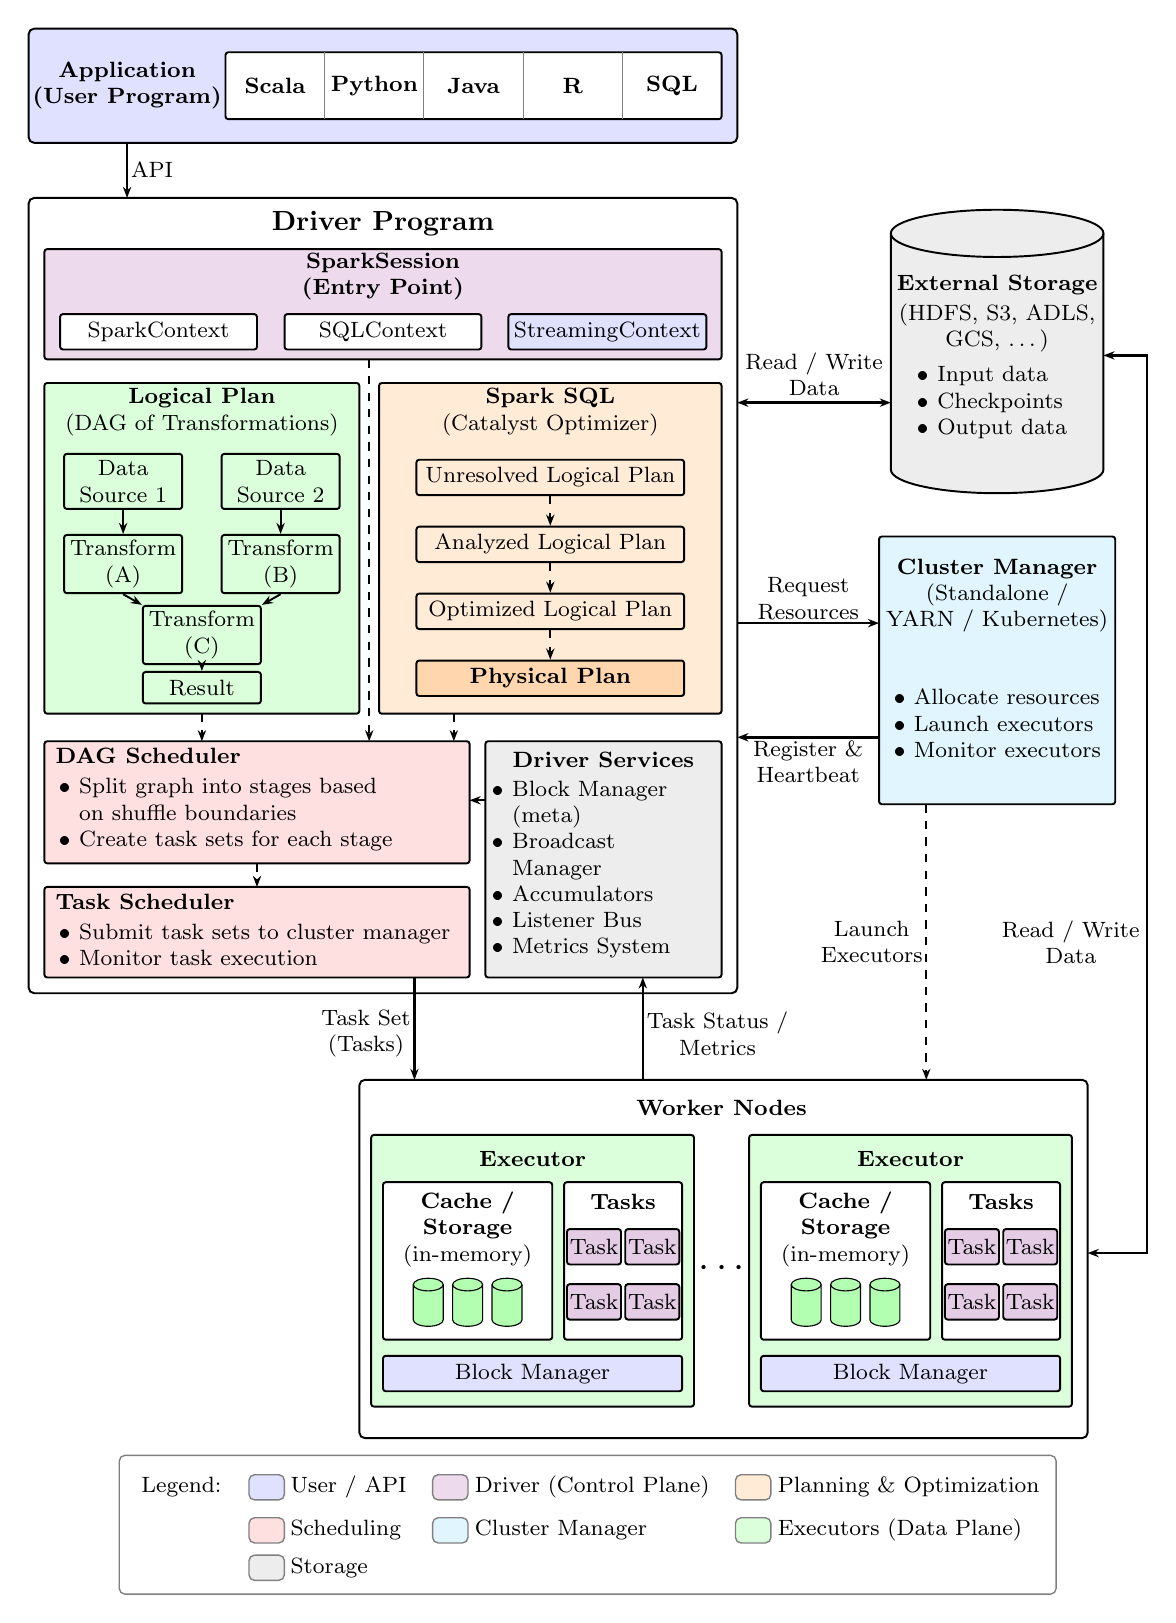
\begin{tikzpicture}[
    every node/.style={font=\footnotesize},
    >={Stealth[length=4pt,width=3pt]},
    box/.style={rectangle,rounded corners=1pt,draw,line width=0.7pt,
      fill=white,align=center,inner sep=2pt},
    frame/.style={rectangle,rounded corners=2pt,draw,line width=0.7pt},
    title/.style={font=\footnotesize\bfseries,align=center,inner sep=1pt},
    bullets/.style={align=left,anchor=north west,inner sep=1pt},
    flow/.style={->,line width=0.9pt},
    dflow/.style={->,line width=0.7pt,dashed},
    lbl/.style={align=center,inner sep=1pt},
    swatch/.style={rectangle,draw,line width=0.5pt,minimum width=0.45cm,
      minimum height=0.32cm,inner sep=0pt},
  ]
  % ==================== Application ====================
  % A strip above the driver program, its languages in a row
  \draw[frame,fill=cuser] (2.8,2.15) rectangle (11.8,0.7);
  \node[title] at (4.05,1.425) {Application\\(User Program)};
  \draw[box,fill=white] (5.3,1.85) rectangle (11.6,1.0);
  \foreach \t [count=\i] in {Scala,Python,Java,R,SQL}
    \node[font=\footnotesize\bfseries] at (5.3+1.26*\i-0.63,1.425) {\t};
  \foreach \i in {1,...,4}
    \draw[line width=0.4pt,gray] (5.3+1.26*\i,1.85) -- (5.3+1.26*\i,1.0);
  \draw[flow] (4.05,0.7) -- node[right,lbl] {API} (4.05,0);

  % ==================== Driver program ====================
  \draw[frame,fill=white] (2.8,0) rectangle (11.8,-10.1);
  \node[title,font=\normalsize\bfseries] at (7.3,-0.32) {Driver Program};

  % ---------- SparkSession ----------
  \draw[box,fill=cdriver] (3.0,-0.65) rectangle (11.6,-2.05);
  \node[title] at (7.3,-1.0) {SparkSession\\(Entry Point)};
  \node[box,minimum width=2.5cm,minimum height=0.45cm] at (4.45,-1.7)
    {SparkContext};
  \node[box,minimum width=2.5cm,minimum height=0.45cm] at (7.3,-1.7)
    {SQLContext};
  \node[box,fill=cuser,minimum width=2.5cm,minimum height=0.45cm]
    at (10.15,-1.7) {StreamingContext};

  % ---------- Logical plan ----------
  \draw[box,fill=cexec] (3.0,-2.35) rectangle (7.0,-6.55);
  \node[title] at (5.0,-2.72) {Logical Plan\\\mdseries(DAG of Transformations)};
  \begin{scope}[every node/.style={box,fill=cexec,font=\footnotesize,
      minimum width=1.5cm,minimum height=0.7cm}]
    \node (ds1) at (4.0,-3.6) {Data\\Source 1};
    \node (ds2) at (6.0,-3.6) {Data\\Source 2};
    \node (ta) at (4.0,-4.65) {Transform\\(A)};
    \node (tb) at (6.0,-4.65) {Transform\\(B)};
    \node (tc) at (5.0,-5.55) {Transform\\(C)};
    \node[minimum height=0.4cm] (res) at (5.0,-6.22) {Result};
  \end{scope}
  \draw[->,line width=0.7pt] (ds1) -- (ta);
  \draw[->,line width=0.7pt] (ds2) -- (tb);
  \draw[->,line width=0.7pt] (ta.south) -- (tc.north west);
  \draw[->,line width=0.7pt] (tb.south) -- (tc.north east);
  \draw[->,line width=0.7pt] (tc) -- (res);

  % ---------- Catalyst ----------
  \draw[box,fill=cplan] (7.25,-2.35) rectangle (11.6,-6.55);
  \node[title] at (9.425,-2.72) {Spark SQL\\\mdseries(Catalyst Optimizer)};
  \begin{scope}[every node/.style={box,fill=cplan,font=\footnotesize,
      minimum width=3.4cm,minimum height=0.45cm}]
    \node (p1) at (9.425,-3.55) {Unresolved Logical Plan};
    \node (p2) at (9.425,-4.4) {Analyzed Logical Plan};
    \node (p3) at (9.425,-5.25) {Optimized Logical Plan};
    \node[fill=orange!32,font=\footnotesize\bfseries] (p4) at (9.425,-6.1)
      {Physical Plan};
  \end{scope}
  \draw[dflow] (p1) -- (p2);
  \draw[dflow] (p2) -- (p3);
  \draw[dflow] (p3) -- (p4);

  % ---------- Schedulers and driver services ----------
  \draw[box,fill=csched] (3.0,-6.9) rectangle (8.4,-8.45);
  \node[title,anchor=north west] at (3.1,-6.95) {DAG Scheduler};
  \node[bullets] at (3.15,-7.33) {\textbullet~Split graph into stages based\\
    \phantom{\textbullet~}on shuffle boundaries\\
    \textbullet~Create task sets for each stage};
  \draw[box,fill=csched] (3.0,-8.75) rectangle (8.4,-9.9);
  \node[title,anchor=north west] at (3.1,-8.8) {Task Scheduler};
  \node[bullets] at (3.15,-9.18) {\textbullet~Submit task sets to cluster
    manager\\\textbullet~Monitor task execution};
  \draw[box,fill=cstore] (8.6,-6.9) rectangle (11.6,-9.9);
  \node[title] at (10.1,-7.13) {Driver Services};
  \node[bullets] at (8.65,-7.36) {\textbullet~Block Manager\\\phantom{\textbullet~}(meta)\\
    \textbullet~Broadcast\\\phantom{\textbullet~}Manager\\\textbullet~Accumulators\\
    \textbullet~Listener Bus\\\textbullet~Metrics System};

  % ---------- Flows inside the driver ----------
  \draw[dflow] (7.125,-2.05) -- (7.125,-6.9);
  \draw[dflow] (5.0,-6.55) -- (5.0,-6.9);
  \draw[dflow] (8.2,-6.55) -- (8.2,-6.9);
  \draw[dflow] (8.6,-7.65) -- (8.4,-7.65);
  \draw[dflow] (5.7,-8.45) -- (5.7,-8.75);

  % ==================== External storage ====================
  \begin{scope}[line width=0.7pt]
    \cyl{15.1}{-0.45}{2.7}{3.0}{0.3}{cstore}
  \end{scope}
  \node[title] at (15.1,-1.1) {External Storage};
  \node[lbl] at (15.1,-1.65) {(HDFS, S3, ADLS,\\GCS, \dots)};
  \node[bullets] at (14.05,-2.1) {\textbullet~Input data\\
    \textbullet~Checkpoints\\\textbullet~Output data};
  \draw[flow,<->] (11.8,-2.6) -- (13.75,-2.6);
  \node[lbl,anchor=south] at (12.775,-2.55) {Read / Write\\Data};

  % ==================== Cluster manager ====================
  \draw[box,fill=ccm] (13.6,-4.3) rectangle (16.6,-7.7);
  \node[title] at (15.1,-5.05)
    {Cluster Manager\\\mdseries(Standalone /\\\mdseries YARN / Kubernetes)};
  \node[bullets] at (13.75,-6.2) {\textbullet~Allocate resources\\
    \textbullet~Launch executors\\\textbullet~Monitor executors};
  \draw[flow] (11.8,-5.4) -- node[above,lbl] {Request\\Resources}
    (13.6,-5.4);
  \draw[flow] (13.6,-6.85) -- node[below,lbl] {Register \&\\Heartbeat}
    (11.8,-6.85);

  % ==================== Worker nodes ====================
  % Below the driver program, its two executors side by side
  \draw[frame,fill=white] (7.0,-11.2) rectangle (16.25,-15.75);
  \node[title] at (11.6,-11.55) {Worker Nodes};
  \foreach \dx in {-11.3,-6.5} {
    \begin{scope}[shift={(\dx,-11.9)}]
      \draw[box,fill=cexec] (18.45,0) rectangle (22.55,-3.45);
      \node[title] at (20.5,-0.3) {Executor};
      \draw[box,fill=white] (18.6,-0.6) rectangle (20.75,-2.6);
      \node[lbl,font=\footnotesize\bfseries] at (19.675,-1.2)
        {Cache /\\Storage\\\mdseries(in-memory)};
      \foreach \c in {19.175,19.675,20.175}
        \cyl{\c}{-1.9}{0.38}{0.45}{0.08}{green!30};
      \draw[box,fill=white] (20.9,-0.6) rectangle (22.4,-2.6);
      \node[title] at (21.65,-0.85) {Tasks};
      \foreach \tx in {21.28,22.02}
        \foreach \ty in {-1.42,-2.12}
          \node[box,fill=violet!20,minimum width=0.62cm,minimum height=0.45cm,
            inner sep=1pt] at (\tx,\ty) {Task};
      \node[box,fill=cuser,minimum width=3.8cm,minimum height=0.45cm]
        at (20.5,-3.03) {Block Manager};
    \end{scope}
  }
  \node[font=\Large] at (11.6,-13.6) {$\cdots$};

  % ---------- Flows of the worker nodes ----------
  \draw[flow] (7.7,-9.9) -- node[left,lbl,pos=0.55] {Task Set\\(Tasks)}
    (7.7,-11.2);
  \draw[flow] (10.6,-11.2) -- node[right,lbl,pos=0.45] {Task Status /\\Metrics}
    (10.6,-9.9);
  \draw[dflow] (14.2,-7.7) -- node[left,lbl] {Launch\\Executors}
    (14.2,-11.2);
  \draw[flow,<->] (16.45,-2.0) -- (17.0,-2.0) -- (17.0,-13.4) --
    (16.25,-13.4);
  \node[lbl,anchor=east] at (16.95,-9.45) {Read / Write\\Data};

  % ==================== Legend ====================
  % Three rows of swatches, centred under the diagram, which spans x = 2.8 to
  % x = 17.0
  \matrix[draw=gray,line width=0.5pt,rounded corners=2pt,inner sep=4pt,
      column sep=0pt,row sep=2pt,
      column 3/.style={nodes={anchor=west}},
      column 5/.style={nodes={anchor=west}},
      column 7/.style={nodes={anchor=west}}]
    at (9.9,-16.85) {
    \node {Legend:}; &[0.2cm]
    \node[swatch,fill=cuser] {}; & \node[inner sep=2pt] {User / API}; &[0.25cm]
    \node[swatch,fill=cdriver] {}; &
      \node[inner sep=2pt] {Driver (Control Plane)}; &[0.25cm]
    \node[swatch,fill=cplan] {}; &
      \node[inner sep=2pt] {Planning \& Optimization}; \\
    &
    \node[swatch,fill=csched] {}; & \node[inner sep=2pt] {Scheduling}; &
    \node[swatch,fill=ccm] {}; & \node[inner sep=2pt] {Cluster Manager}; &
    \node[swatch,fill=cexec] {}; &
      \node[inner sep=2pt] {Executors (Data Plane)}; \\
    &
    \node[swatch,fill=cstore] {}; & \node[inner sep=2pt] {Storage}; &
    & & & \\
  };
\end{tikzpicture}
\end{document}
